\section{Algoritmos de Composición}
\label{sec:algComposicion}

\todo{ Revisar y reestructurar}\\

En esta sección se explicará de forma exhaustiva los procesos que se siguen para componer música a partir de los datos que nos proporciona el análisis de imagen.\\

Para generar la música separamos el proceso de composición en diferentes voces, de tal modo que la unión de todas las voces da como resultado una pieza musical completa. En el estado actual del proyecto se ha identificado cuatro voces diferentes cada una con un papel especial dentro de la composición. 

Cada voz sigue un proceso de composición independiente aunque concuerdan en algunos aspectos para poder realizar una unión correcta de todas ellas, como por ejemplo, la duración total de las mismas. Todos los compositores de forma imprescindible reciben una figura, en la que se van a basar para componer, y una duración dada que será el tiempo que se prolonga el trozo de música a componer.\\

A continuación se explicará el funcionamiento de los algoritmos de cada voz y al final se presentará el algoritmo que se encarga de ir usando cada una de las voces.

%----------------------------------------------------------------------------------------------------------------------------------------------------
\subsection{1ª Voz: Melodía Principal}

Normalmente en una composición suele haber una voz que destaca sobre las demás, que es la que el oído reconoce primero. Esta voz reproduce la melodía. Para poder crear la melodía, vamos a componer a nivel de notas y la relación entre ellas. En nuestro caso, una nota se separa en dos dimensiones: duración y tono. Siguiendo esta separación se ha dividido el proceso de composición en cuatro fases: procesar la figura, calcular duraciones, obtener tonos y sintetizar o unir las duraciones con los tonos.\\
Para voz principal se ha dejado la posibilidad de elegir entre dos versiones diferentes del compositor. La primera que se desarrolló tiene algunos pequeños defectos que luego en la segunda versión del compositor se corrigieron.\\

La primera versión (ComposerFigMelody):
\begin{itemize}
	\item Procesar la figura: El algoritmo de entrada dispone de una figura, en la que se va a basar más adelante para componer. Antes hace falta un proceso de normalización para que todas las figuras puedan ser interpretadas correctamente. Para ello se saca los vértices ordenados de la figura de tal forma que el primer vértice sea el más alto de la figura y los siguientes estén en sentido horario. Además, durante el proceso, se irá calculando la longitud de los lados de la figura.

	\item Calcular duraciones: Para poder obtener las duraciones de las futuras notas se hace una correpondencia directa con la longitud de los lados. De este modo la duración total del trozo de música a componer es la suma de todas la longitudes y para cada lado se calcula cuanta duración le corresponde. Obviamente se hace una aproximación ya que los valores de duración de las notas son limitados respecto al rango de valores de los números reales.

	\item Obtener tonos: Hallamos los tonos a partir de los ángulos de la figura. En otros trabajos se han explorado diferentes maneras de conseguirlo(\cite{bricksConvertsMusic} \cite{ImageBaseComposition}). El proceso de cálculo de tono se basa en la idea de estabilidad e inestabilidad que se desarrolla en el trabajo de A. Pintado (\cite{portutesis}). Una figura es estable cuanto más suave sea su contorno, es decir, cuantos menos picos, ángulos diferentes e irregularidades tenga. A. Pintado usa esta cualidad para generar ritmos a partir de figuras y líneas, aquí se va a usar para calcular tonos. De tal modo que un ángulo más abierto implica mayor cambio en el tono y viceversa.
En la tercera fase, en vez de usar un algoritmo diferencial donde se tiene en cuenta la variación respecto al anterior ángulo examinado, se usa una correspondencia directa donde: cuanto mayor sea el ángulo mayor será el salto de tono. Además el signo del ángulo determina la dirección del salto (Figura~\ref{fig:Figura6Voz1}).

\end{itemize}
----------
A continuación, en la segunda fase, se calculan la longitud media de los lados, el lado más largo y el lado más corto. Se asignan duraciones a cada lado teniendo en cuenta sus longitudes.Se utilizan las duraciones simples de las notas en música: blancas, negras, corcheas, semicorcheas... como aproximación de las longitudes obtenidas en lugar de las compuestas que permitirían una equivalencia perfecta entre la longitud de los lados y la duración de las notas. Puede parecer preferible conseguir la equivalencia perfecta entre longitud y duración, sin embargo, tras varias pruebas  (Figura~\ref{fig:Figura5Voz1}) no se ha conseguido un resultado que cumpliese esa propiedad y al mismo tiempo no perdiese el concepto de ritmo musical.\\

		\begin{figure}[htbp]
		\centering
		\hspace*{0.0in}
		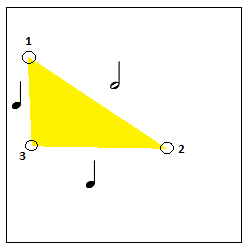
\includegraphics[scale=1.0]{graphics/simpletest1-F2.png}
		\caption{Figura de entrada con el ritmo producido}
		\label{fig:Figura2Voz1}
		\end{figure}

En el ejemplo (Figura~\ref{fig:Figura2Voz1}) se puede apreciar cómo el lado más largo obtiene una duración mayor (blanca) que los otros dos lados (negra). A pesar de que los dos lados más pequeños tienen diferentes longitudes, se ha aproximado su longitud a una misma duración.\\

\todo{A que te refieres con una figura es estable? -> solved?}
La tercera fase se centra en obtener los tonos de las notas que se van a crear. En otros trabajos se han obtenido de diferentes manera(\cite{bricksConvertsMusic} \cite{ImageBaseComposition}). La aproximación que se usa en este proyecto se basa en la idea de estabilidad e inestabilidad que se desarrolla en el trabajo de A. Pintado (\cite{portutesis}). Una figura es estable cuanto más suave sea su contorno, es decir, cuantos menos picos, ángulos diferentes e irregularidades tenga. A. Pintado usa esta cualidad para generar ritmos a partir de figuras y líneas, aquí se va a usar para calcular tonos.\\

\todo{El diferencial del ángulo esta bien dicho? -> solved}
La obtención de los tonos viene de los ángulos de las figuras, para ello se coge el primer vértice y se calcula su ángulo. Por ser la primera nota le asignamos el tono correspondiente al color de la figura dentro del sistema de colores usado (p. ej: Rojo en el sistema Scriabin es C ``do'', amarillo es D ``re''...). A partir de ahí, dependiendo de cuánto ha variado el ángulo del siguiente vértice respecto al anterior, vamos asignando un tono más alto o más bajo según sea positivo o negativo la diferencia de ángulos.

\todo{y la cantidad de tonos que debe variar el nuevo tono: no hay otra manera de expresarlo? es redundante. Aparte la frase me suena raro pero no veo otra forma de decirlo  -> solved?}
De forma experimental y tras varias pruebas, se ha obtenido una correspondencia entre la variación de ángulos y la cantidad que deberá variar el nuevo tono respecto al anterior (Figura~\ref{fig:Figura3Voz1}). 

		\begin{figure}[htbp]
		\centering
		\hspace*{0.0in}
		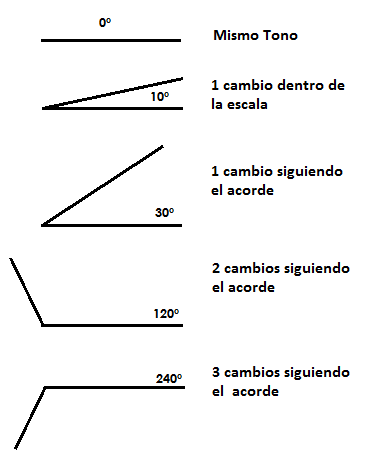
\includegraphics[scale=0.75]{graphics/tabla-corresp-Tono-Angulo.png}
		\caption{Tabla correspondencias entre ángulos y cambios de tono}
		\label{fig:Figura3Voz1}
		\end{figure}

\todo{En cuanto a lo de se usa el tono vecino no sería mejor decir algo como: se usa uno de los tonos adyacentes dentro de la escala cromática. no se, con lo del tono vecino no queda claro lo que quieres decir -> solved\\
Del acorde del color de la figura: no hemos hablado de acordes hasta ahora, a que te refieres?\\
Qué es el acorde fundamental, está explicado en alguna otra parte?\\
No entiendo esta frase: Se usa el acorde fundamental con tono fundamental la nota del color de la figura para los grandes saltos porque conseguimos notas consonantes con el color de la figura. -> cambiada\\
Habrá que mencionar la escala cromática en algún lado, referencia?}
De este modo si la diferencia de ángulos es menor a 10º se sigue usando el mismo tono, si la diferencia está entre 10º y 30º se usa el tono adyacente dentro de la escala, si está entre 30º y 120º el segundo tono más cercano del acorde, entre 120º y 240º el segundo tono más cercano del acorde y hasta 360º el tercer tono más cercano del acorde. El acorde que se usa es el acorde fundamental del tono que da el color de la figura. Esta relación se basa en la asociación que tiene Scriabin con los colores(\cite{ScriabinQuintasColor}), él hacía corresponder un color a un tono y a su acorde fundamental sin distinguir entre acorde mayor o menor para cada una de las notas de la escala cromática.

\todo{Su estabilidad es muy alta creo que haces referencia a lo de la portutesis, no habría otra manera de decirlo que sea mas simple: la variación de sus ángulos es constante o algo así ->solved?}
De esta manera se consigue que en una figura simétrica con todos sus ángulos iguales sea una figura muy estable y por tanto suena la misma nota. Normalmente el círculo sería la figura de mayor estabilidad y se correspondería a una nota de larga duración, pero, por el proceso de análisis, el círculo se aproxima a un polígono regular de muchos lados y por tanto a muchas notas con el mismo tono.

		\begin{figure}[htbp]
		\centering
		\hspace*{0.0in}
		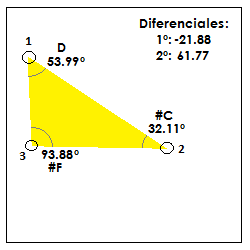
\includegraphics[scale=1.0]{graphics/simpletest1-F3.png}
		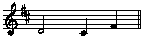
\includegraphics[scale=1.0]{graphics/simpletest1-MELpartitura.png}
		\caption{Figura de entrada con los ángulos y los tonos que produce}
		\label{fig:Figura4Voz1}
		\end{figure}

\todo{No se entiende bien que pasa aquí: se sube de un salto en el acorde de nota fundamental el color de la figura\\
primero hablas de saltar tonos y luego al final de este párrafo dices dar el salto de una nota -> Eso es que de la nota re, das un salto a fa, que es la siguiente nota dentro del acorde(re-fa-la). Nose creo que eso para explicarlo mejor tengo que bajar a muy bajo nivel. Si se sabe que es acorde, no debería de haber problema.}
Como se puede observar en el ejemplo (Figura~\ref{fig:Figura4Voz1}), se tienen los 3 ángulos con su nota correspondiente ya calculada. Para conseguirlo primero se tiene que ver qué nota corresponde al color de la figura (en este caso se usa la correspondencia propuesta por Scriabin en la que el amarillo es D ``re''). Una vez se tiene la nota y su ángulo, se calcula la diferencia entre el nuevo ángulo y el anterior, el resultado es negativo por lo que se tiene que bajar de tono y como la diferencia está entre los 10º y 30º, sólo se baja un escalón en la escala actual (en este ejemplo la de Re Mayor), obteniendo la nueva nota: C ``do''. Para conseguir el último tono, se calcula el diferencial del último vértice restando el ángulo del tercer vértice con el del segundo. Se obtiene un valor positivo, luego se tiene que subir el tono, all estar entre 30º y 120º se sube de un salto en el acorde de nota fundamental el color de la figura (en este caso es el acorde de D ``re'': D - F ``fa''- A ``la''). Cómo no se está en el acorde con el último tono obtenido (C ``do'') se viaja al tono más cercano que pertenezca al acorde, es decir, D ``re''. Y de ahí se da un salto dentro del acorde y como el ángulo es positivo se salta a la nota superior: F ``fa''.

Por último, la cuarta fase se encarga de combinar las duraciones con los tonos para crear las notas. Al final se obtiene un trozo de música de una de las voces (Partitura de Figura~\ref{fig:Figura4Voz1}).
\todo{El ejemplo quizas haciendolo más esquemático quedaría más claro, ahora mismo es bastante lioso -> Se podrían poner más imágenes con pasos intermedios, pero podrían pensar que estamos engordando la memoria}

\todo{Esto está mal estructurado, empiezas hablando de la composición musical en general pero de repente tras contar el ejemplo dices que es de tal compositor, debería de ser mas al estilo del analizador de figuras, hablas de las 4 fases de la composición y luego dices compositor tal: fase uno asi y asi, fase dos asa y asa etc..., y si eso el ejemplo para ayudar a entenderlo, luego compositor cual: asi y asa... etc... ahora mismo con este salto se vuelve todo lioso y uno falla en ver la estructura del tema\\
A partir de o unidades más pequeñas... al final del parrado, no se entiende a que te refieres}
Este algoritmo está implementado en la clase ComposerFigMelody2. Además hay otro compositor, ComposerFigMelody, que se desarrolló durante las primeras pruebas de composición, que trabaja de manera diferente en la segunda y tercera fase. En la segunda fase, al hacer corresponder las duraciones con las longitudes de los lados se usan las duraciones compuestas (buscando la máxima exactitud entre longitud de lado y duración) siendo la unidad mínima indivisible la semicorchea o unidades más pequeñas si la duración pedida del segmento de música es especial (no divisible en semicorcheas) (Figura~\ref{fig:Figura5Voz1}).

		\begin{figure}[htbp]
		\centering
		\hspace*{0.0in}
		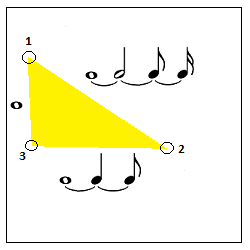
\includegraphics[scale=1]{graphics/simpletest1-F2_2.png}
		\caption{Figura de entrada con los lados y el ritmo conseguido}
		\label{fig:Figura5Voz1}
		\end{figure}

En la tercera fase, en vez de usar un algoritmo diferencial donde se tiene en cuenta la variación respecto al anterior ángulo examinado, se usa una correspondencia directa donde: cuanto mayor sea el ángulo mayor será el salto de tono. Además el signo del ángulo determina la dirección del salto (Figura~\ref{fig:Figura6Voz1}).

		\begin{figure}[htbp]
		\centering
		\hspace*{0.0in}
		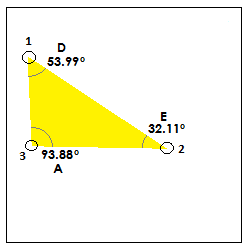
\includegraphics[scale=1]{graphics/simpletest1-F3_2.png}
		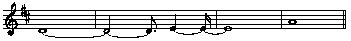
\includegraphics[scale=1]{graphics/simpletest1_2-MELpartitura.png}
		\caption{Figura de entrada con los ángulos y los tonos producidos}
		\label{fig:Figura6Voz1}
		\end{figure}

%----------------------------------------------------------------------------------------------------------------------------------------------------

\subsection{2ª Voz: Melodía Secundaria}

\todo{A estas alturas debes odiarme: El tema de la adaptación no queda nada claro...}
Para crear la segunda voz que sirve de acompañamiento a la primera, se usa la misma estructura que a la hora de componer la melodía principal, aunque también se necesita el segmento de melodía principal como entrada para poder basarse en ella para componer. 
La primera fase es igual que en la primera voz. La segunda fase también es igual salvo que al final se introduce un paso de adaptación. Debemos hacer una adaptación de la duración del total obtenido al analizar la figura (Figura~\ref{fig:Figura1Voz2} sin adaptar y Figura~\ref{fig:Figura2Voz2} con adaptación). Eso ocurre ya que se quiere que el segmento de música que se genera tenga una duración determinada menor o igual a la melodía principal. Además se debe decidir en qué momento de la melodía principal se empieza a decorar introduciendo así la segunda voz.

 		\begin{figure}[htbp]
		\centering
		\hspace*{0.0in}
		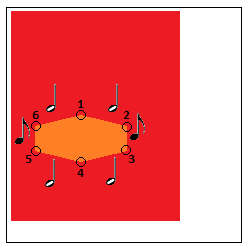
\includegraphics[scale=1]{graphics/simpletest4-F2.png}
		\caption{Figuras de entrada con los lados de la figura interior y las duraciones obtenidas sin adaptación}
		\label{fig:Figura1Voz2}
		\end{figure}

		\begin{figure}[htbp]
		\centering
		\hspace*{0.0in}
		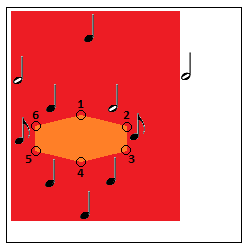
\includegraphics[scale=1]{graphics/simpletest4-F2_2.png}
		\caption{Figuras de entrada con la duración de la figura exterior y con las duraciones adaptadas de la interior}
		\label{fig:Figura2Voz2}
		\end{figure}

\todo{No sería conveniente explicar esto antes de explicar que se adapta? ademas habría que estructurar todo esto por fases como mencioné anteriormente, esta todo muy caótico}
Esta función de adaptación se encarga de ir dividiendo a la mitad diferentes duraciones para reducir la duración total del segmento (o ir aumentando, duplicando duraciones, si se necesita aumentar la duración total). 

\todo{Vale... en lugar de decir cambios y luego decir cambios siguen principios de, y luego cambios se activan en habría que ponerlo de manera que sea, por ejemplo: mientras se genera el acompañamiento se va analizando el resultado para cambiar el tono subiendo o bajando a una nueva nota de tal manera que la melodía cumpla las reglas contrapuntísticas más básicas consiguiendo un acompañamiento que no sea disonante con la melodía principal}
El otro cambio se hace en la tercera fase. Mientras se generan los tonos se analiza el comportamiento de la segunda voz respecto a la melodía principal. Este paso es necesario para disminuir las disonancias que puedan aparecer al juntar ambas voces (Figura~\ref{fig:Figura3Voz2}). Por ello mientras se genera la nueva melodía se van haciendo pequeños cambios en la segunda voz que lleven a un resultado mejorado. Los cambios usados siguen los principios de las técnicas más básicas contrapuntísticas. Estos cambios se activan cuando el intervalo entre la voz primera y la voz segunda es disonante y se mantiene un periodo alargado en el tiempo (igual o mayor a la duración media de las notas, normalmente una negra). Cómo se intenta minimizar los cambios, se suele hacer que si el cambio de tono era para subir, se sube menos o más el nuevo tono dependiendo de qué implica un menor cambio. Lo mismo cuando el cambio de tono es para bajar, se baja un poco más o menos el nuevo tono (Figura~\ref{fig:Figura3Voz2}).

		\begin{figure}[htbp]
		\centering
		\hspace*{0.0in}
		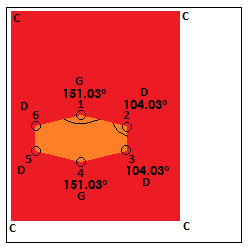
\includegraphics[scale=1]{graphics/simpletest4-F3.png}
		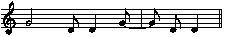
\includegraphics[scale=1]{graphics/simpletest4-F3-MEL2partitura.png}
		\caption{Figuras de entrada con los ángulos y los tonos producidos sin técnicas contrapuntísticas}
		\label{fig:Figura3Voz2}
		\end{figure}

		\begin{figure}[htbp]
		\centering
		\hspace*{0.0in}
		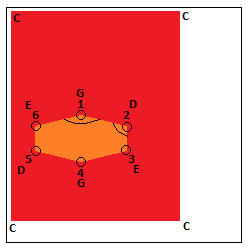
\includegraphics[scale=1]{graphics/simpletest4-F3_2.png}
		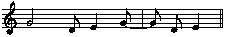
\includegraphics[scale=1]{graphics/simpletest4-F3_2-MEL2partitura.png}
		\caption{Figuras de entrada con los ángulos y los tonos producidos con técnicas contrapuntísticas}
		\label{fig:Figura4Voz2}
		\end{figure}

En la mayoría de ocasiones, el segmento de la segunda voz tiene una duración menor que el segmento de primera voz a la que va acompañando, esto ocurre porque normalmente la figura de entrada es menor que la figura que se usó para componer la melodía principal. Para que el segmento de la segunda voz tenga la misma duración se rellenan los huecos antes y después del trozo de melodía compuesto con silencios.

%----------------------------------------------------------------------------------------------------------------------------------------------------

\subsection{3ª Voz: Bajo}

Para el bajo, el algoritmo consiste en usar siempre notas de una misma duración (por defecto redondas) cuyo tono sea el color de la figura de entrada y cuya duración sea la de la figura dada (Figura~\ref{fig:Figura1Voz3}).

		\begin{figure}[htbp]
		\centering
		\hspace*{0.0in}
		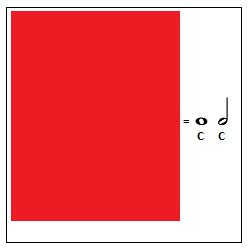
\includegraphics[scale=1]{graphics/simpletest2-F2F3.png}
		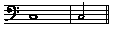
\includegraphics[scale=1]{graphics/simpletest2-BASSpartitura.png}
		\caption{Figura de entrada con los tonos producidos}
		\label{fig:Figura1Voz3}
		\end{figure}

\todo{Solo tienes en cuenta el transportar la melodía dos octavas más grave, este fallo no se puede expresar de manera más general?}
Otra posibilidad disponible para el bajo es usar la el algoritmo de la primera voz pero transportando los tonos una o varias octavas más abajo (Figura~\ref{fig:Figura2Voz3}). El número de octavas depende del tono más agudo y del tono más grave de la melodía compuesta hasta el momento. Si al transportar la melodía a dos octavas más grave se sale del límite de representación de las notas, entonces sólo se transportara una octava más grave.

		\begin{figure}[htbp]
		\centering
		\hspace*{0.0in}
		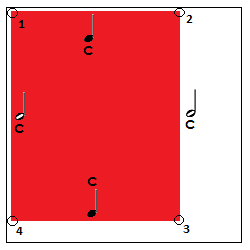
\includegraphics[scale=1]{graphics/simpletest2-F2F3_2.png}
		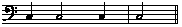
\includegraphics[scale=1]{graphics/simpletest3_2-BASSpartitura.png}
		\caption{Figura de entrada con los tonos producidos}
		\label{fig:Figura2Voz3}
		\end{figure}

%----------------------------------------------------------------------------------------------------------------------------------------------------

\subsection{4ª Voz: Ritmo}

\todo{Estructuración: primera version: blah blah blah, segunda versión: blah balh\\
Que es dividir la figura en varias secciones de ángulos? no se podría decir: se divide la figura de tal manera que cada vértice queda dentro de una sección?\\
Que son las proporciones?\\
A que  se refiere la duración dada por la entrada, no has mencionado en ningún sitio que se diese una duración al algoritmo}
Para el ritmo hay una primera versión basada en la disposición de los vértices. Se divide la figura en varias secciones de ángulos dejando los vértices en diferentes secciones. Estas secciones son configurables de tal manera que se pueden cambiar las proporciones. Una vez se tienen los vértices de cada sección, se sustituyen por ritmos de tal modo que si no hay un vértice en una sección se coloca un silencio y si hay un vértice entonces se coloca un pulso de ritmo (Figura~\ref{fig:Figura1Voz4}). Este ritmo se repite durante la duración dada por entrada.

		\begin{figure}[htbp]
		\centering
		\hspace*{0.0in}
		
\includegraphics[scale=0.57]{graphics/todo.png}
		\caption{Figura de entrada y los ritmos producidos}
		\label{fig:Figur1Voz4}
		\end{figure}

\todo{una serie de vértices dependiendo de la densidad de vertices de la figura? a que se refiere?\\
no entiendo nada del tema de desviación respecto al circulo del área igual a la figura... igualmente, aparte de expresar eso bien tendría que estar más estructurado, se me ocurre algo en plan: las notas dependerán de dos elementos: los vertices y el punto de equilibrio. la relación con los vértices se produce cuando... la relación con el punto de equilibrio se calcula de la siguiente manera... al juntar ambos calculos los vertices producen blah y el punto de equilibrio bleh consiguiendo asi un ritmo blah blah}
El otro ritmo implementado se basa en el concepto de inestabilidad de una figura de A. Pintado (\cite{portutesis}). Por defecto se crea un ritmo que consiste en pulsos largos de duración configurable. A cada nota le es asignada una serie de vértices dependiendo de la densidad de vértices de la figura. Después se va calculando cuanta desviación producen esos vértices respecto al círculo de área igual a la figura y con centro el punto de equilibrio de la figura (Figura~\ref{fig:Figura2Voz4}). A mayor desviación, mayor inestabilidad luego el ritmo se subdivide en más notas de menor duración (Figura~\ref{fig:Figura3Voz4}).

		\begin{figure}[htbp]
		\centering
		\hspace*{0.0in}
		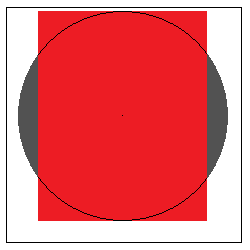
\includegraphics[scale=1]{graphics/simpletest2-Circulo.png}
		\caption{Figura de entrada y el círculo equivalente}
		\label{fig:Figura2Voz4}
		\end{figure}

		\begin{figure}[htbp]
		\centering
		\hspace*{0.0in}
		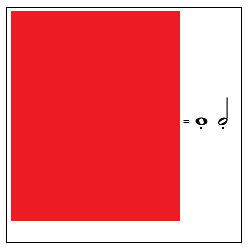
\includegraphics[scale=1]{graphics/simpletest2-F2F3_3.png}
		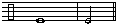
\includegraphics[scale=1]{graphics/simpletest2-PERpartitura.png}
		\caption{Figura de entrada y los ritmos producidos}
		\label{fig:Figura3Voz4}
		\end{figure}

%----------------------------------------------------------------------------------------------------------------------------------------------------

\subsection{Mixer}

\todo{Sería conveniente cambiar mixer por algún tecnicismo}
Los anteriores algoritmos sirven para crear un trozo de música de una voz a partir de una figura, el siguiente paso es juntar las distintas voces para formar una melodía, para ello se utiliza el ``Mixer''

\todo{En una primera implementacion? ya no se hace así? si es el caso para que esta mencionado aqui?, aparte lo de siempre estructurar las cosas, al mencionar las características se puede hacer una lista etc... y cambiar todos los tonos personales como cambiamos a se cambia, aparte lo mismo de antes estructura, se podría poner: mezclador, se encarga de blah balh,en el proyecto se usan dos mezcladores: mezclador uno: blah balh, Mezclador 2: blah blah y demás...}
En una primera implementación el Mixer se encargaba de ordenar las figuras en orden de relevancia siguiendo el parámetro de vistosidad calculado a partir de tres características de la figura.
La primera es lo vistosidad del color de la figura. Para ello descomponemos el color en sus tres componentes principales RGB y damos peso a cada uno de ellos y lo multiplicamos por la saturación del color.
La segunda componente es el área que ocupa la figura. Cuanto más grande sea, más vistosa es.
La tercera componente es la distancia que tiene del centro de la imagen. El ojo humano enfoca de centro a laterales cuando ve una imagen por primera vez, por ello tiene más vistosidad una figura que se encuentra en el centro de la imagen que en un lateral.

	\begin{center}
		$vistosidad(Figura) =$
	\end{center}
	\begin{center}
		
		$\left\{
		\begin{array}{cc}
		A = 0.5f; B = 0.3f; C = 0.2f;\\ 
		pR = 0.45f; pG = 0.35f; pB = 0.20f;\\
		A*getSaturation()*(rgb.r*pR + rgb.g*pG + rgb.b*pB)\\
		 + B*area + C*distanceCenter
		\end{array}\right.$
	\end{center}

Tras haber ordenado las figuras por vistosidad vamos componiendo con cada una de forma iterativa las distintas voces. En el primer Mixer que hicimos, sólo se componía  de melodía y ritmo. Para la segunda versión del Mixer se sigue calculando la vistosidad como se explicó pero en vez de ordenar todas las figuras, ordenamos solo las figuras que están en la imagen sin estar dentro de otra figura, las llamadas figuras padre. Una vez las tenemos vamos iterando por cada figura padre componiendo su melodía, bajo y ritmo. Si la figura padre tiene otras figuras dentro de ella (figuras hijas), entonces también se añade la segunda melodía dando como entrada al algoritmo de composición de acompañamiento esta segunda figura (la figura hija). Por cada figura interior se compone un nuevo bloque de la figura padre con diferentes acompañamientos (Figura~\ref{fig:Figura1Mixer}).

		\begin{figure}[htbp]
		\centering
		\hspace*{0.0in}
		
\includegraphics[scale=1]{graphics/simpletest5.png}
		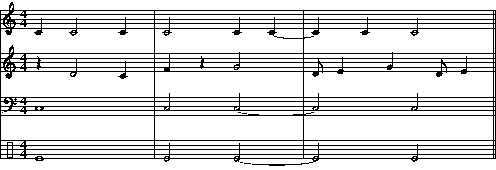
\includegraphics[scale=1]{graphics/simpletest5-partitura.png}
		\caption{Figuras de entrada las voces producidas}
		\label{fig:Figura1Mixer}
		\end{figure}

Una vez tenemos compuestas todas las voces, es el Mixer el que se encarga de juntarlas y llamar a la creación de la partitura y posterior conversión a midi.
